\section{Results}

\begin{figure}
    \centering
    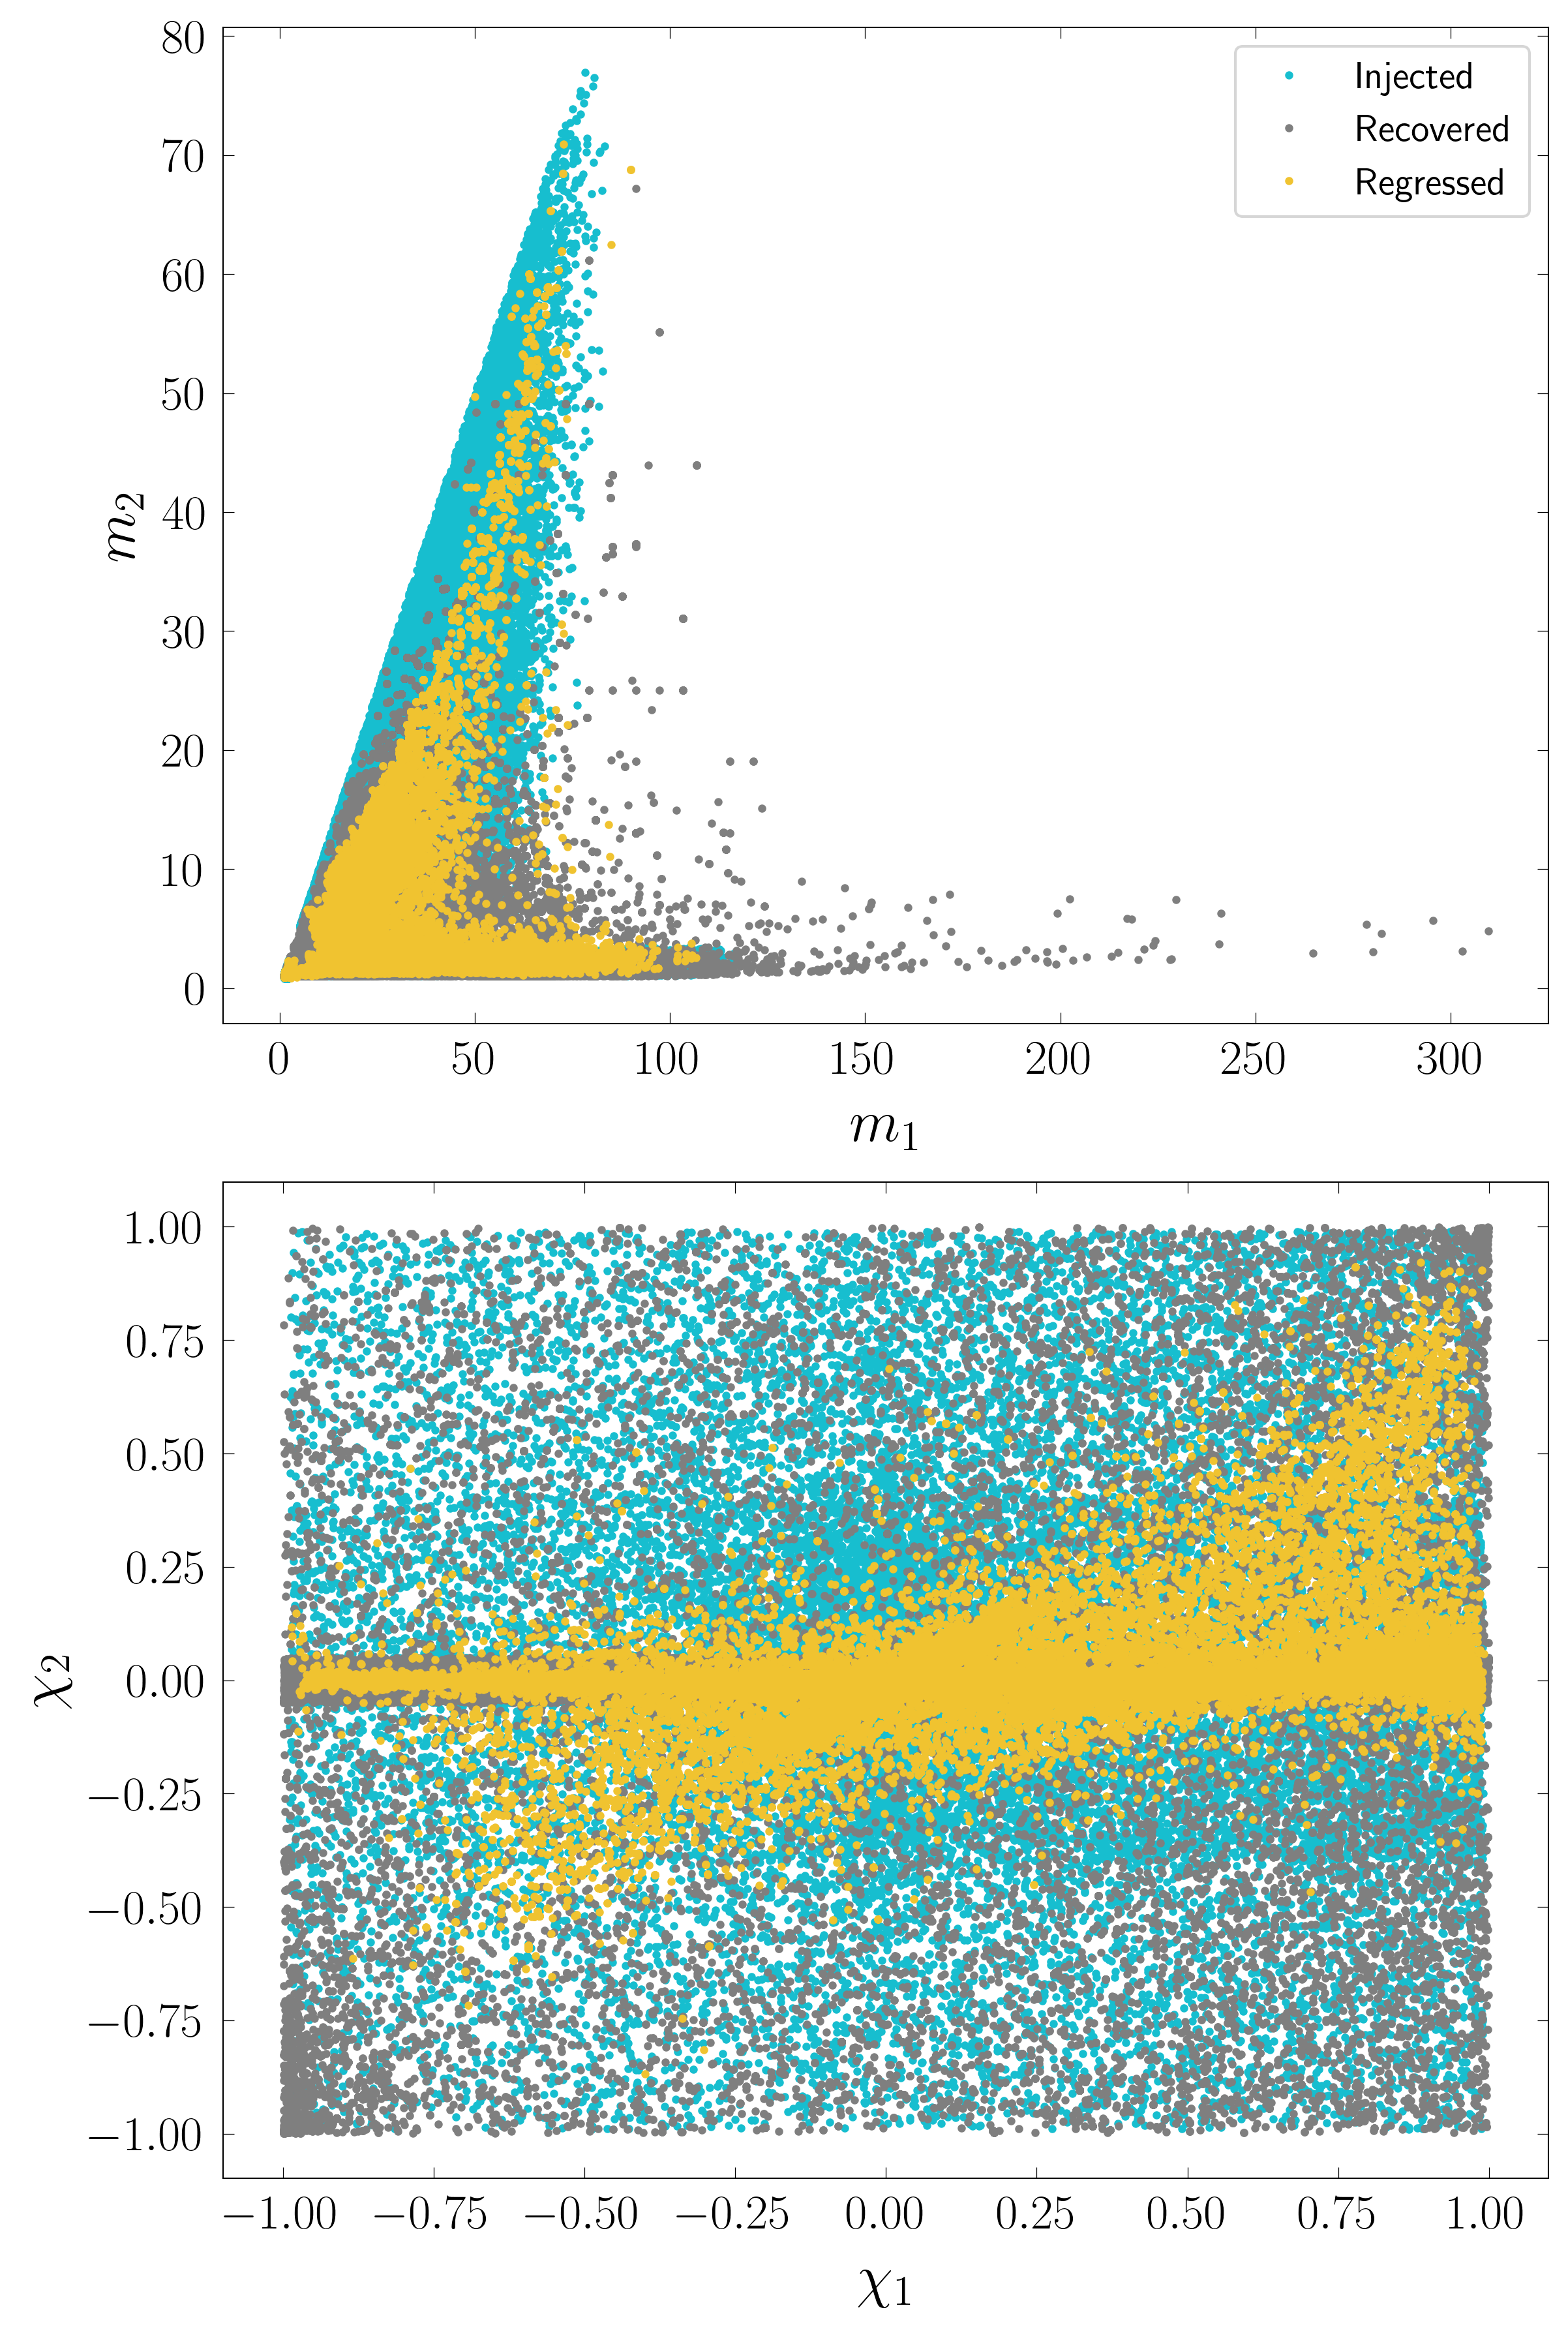
\includegraphics[width=0.45\textwidth]{inj_rec_pred_masses.png}
    \caption{The top panel shows the mass parameter space while the 
    		bottom panel shows the spin parameter space for the 
		injected (teal), recovered (gray), and regressed (yellow) 
		quantities. The regressed quantities shown here are using GPR.
            }
        \label{inj_rec_pred_masses}
\end{figure}

\begin{figure*}[t]
    \centering
    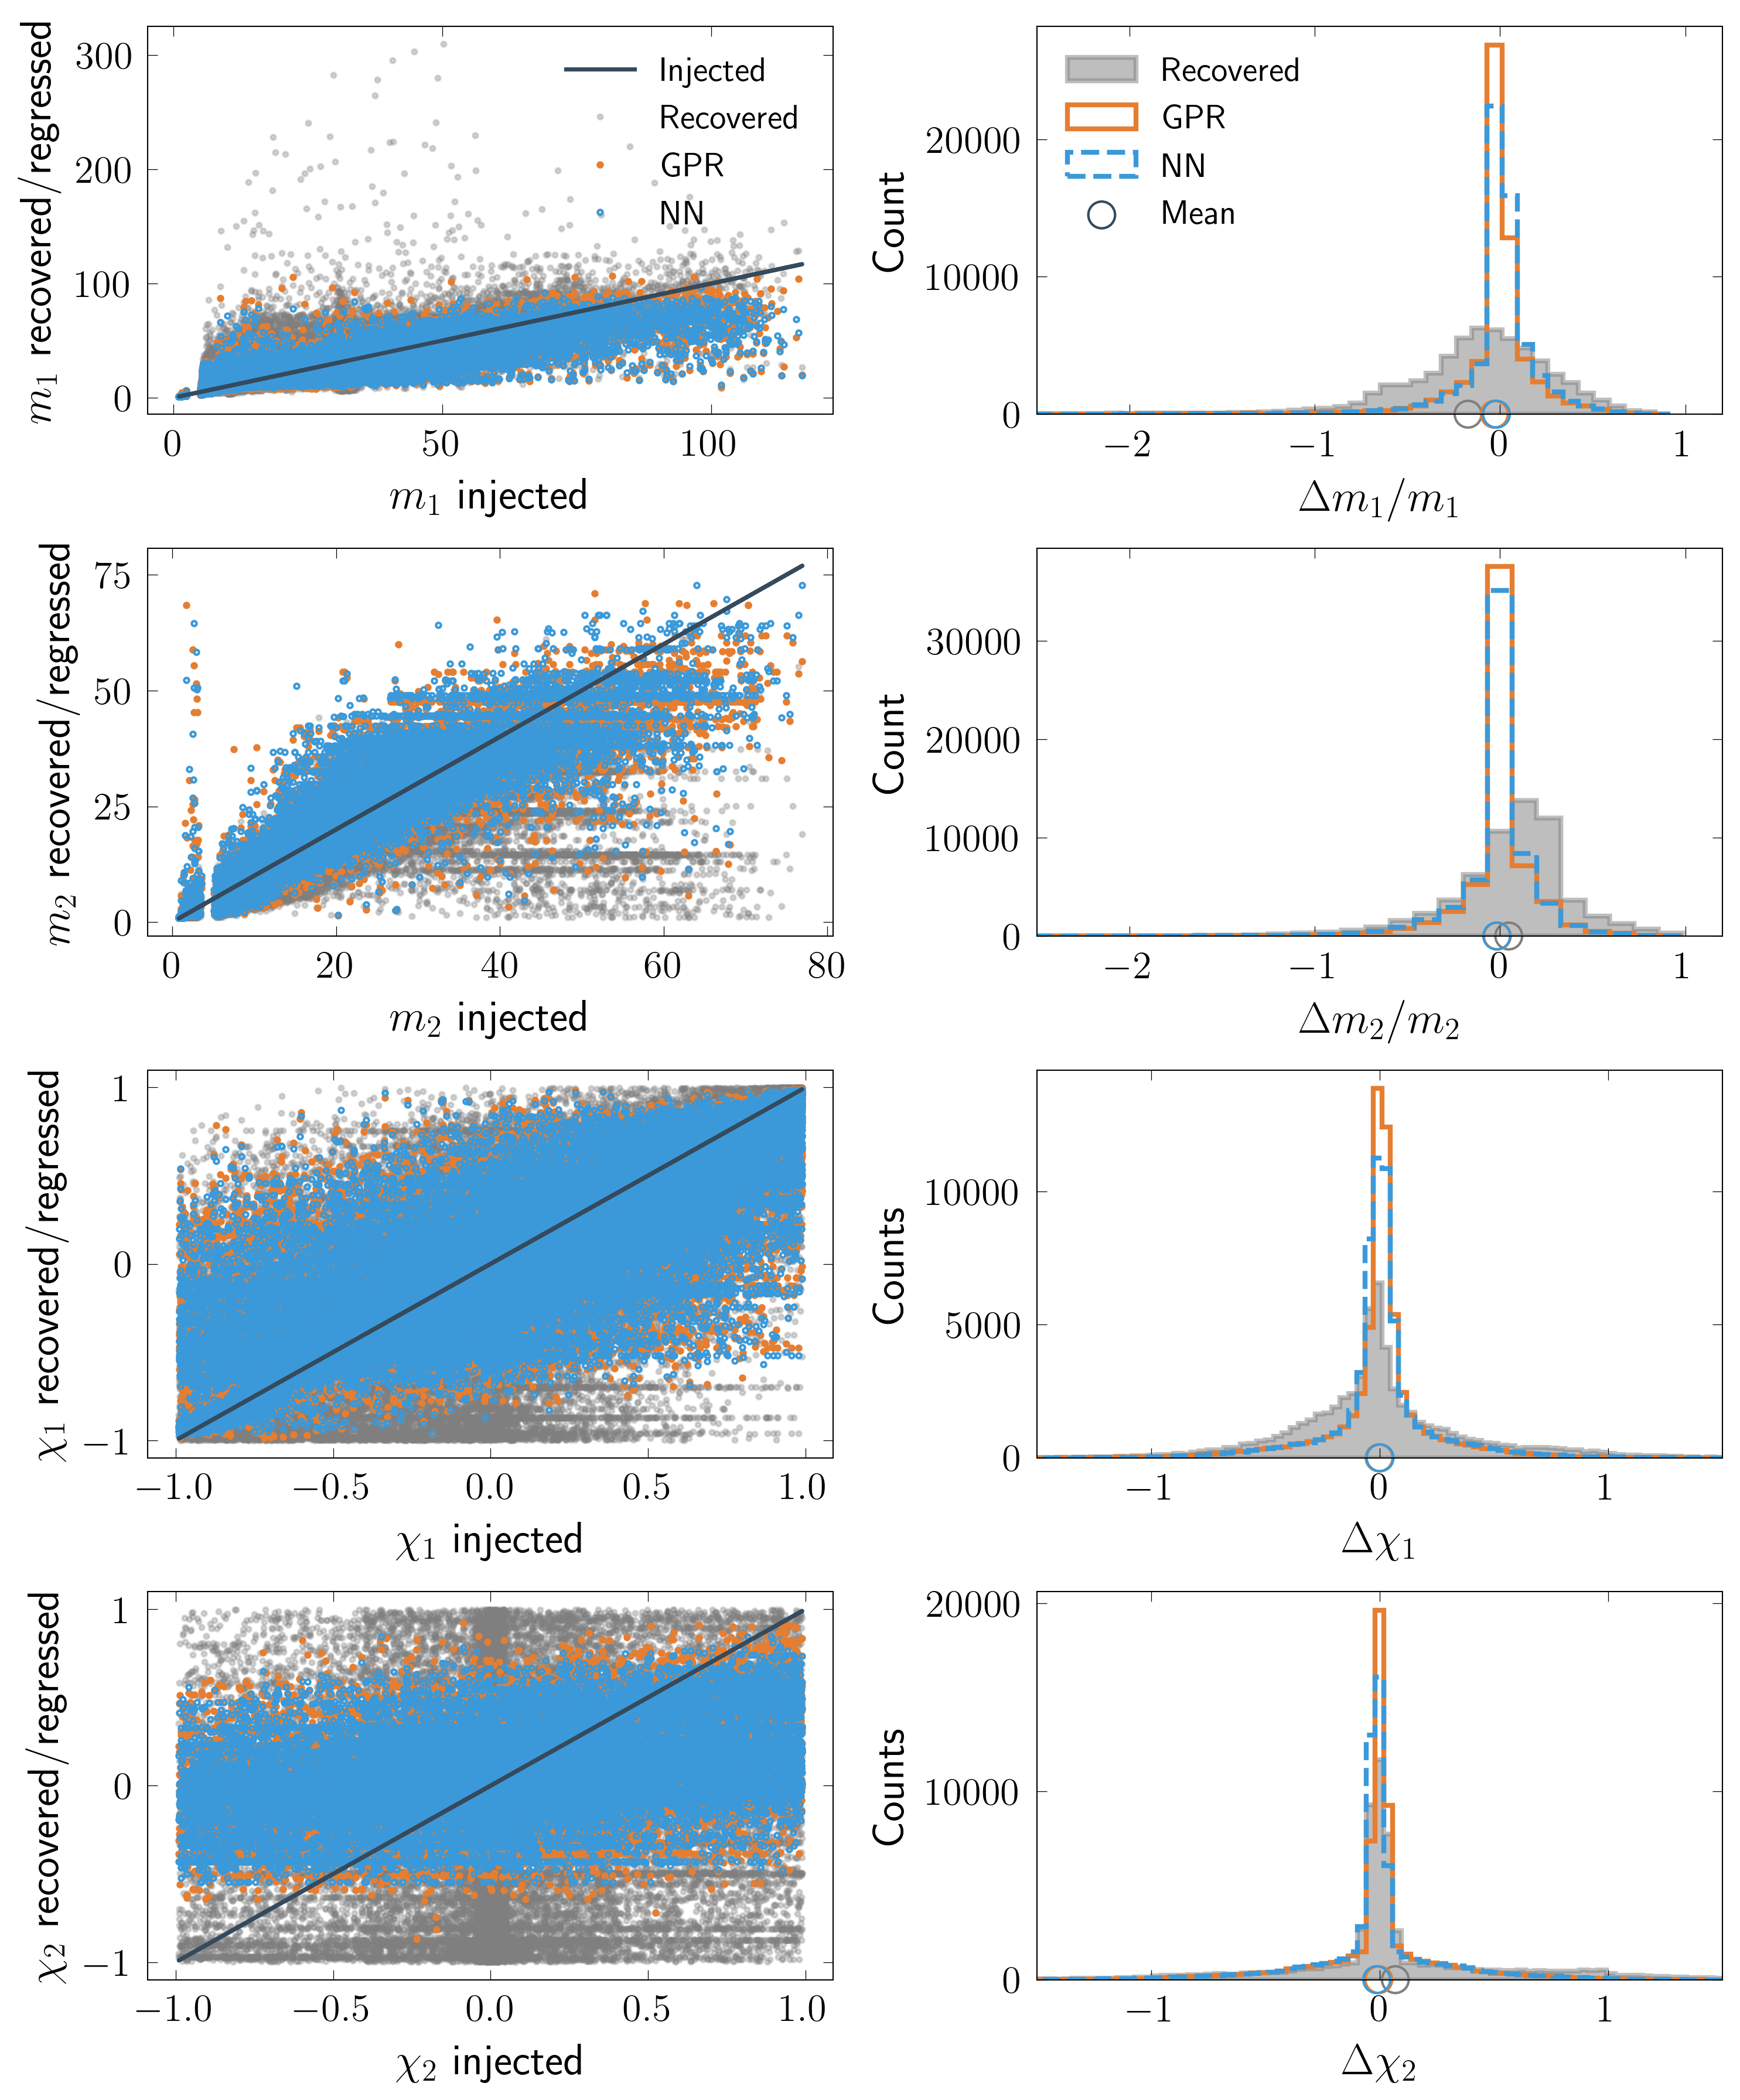
\includegraphics[width=\linewidth]{GPRvsNN_with_hist.png}
    \caption{The left side panels show the recovered (gray) and regressed
             masses and spins as functions of the injected values (solid line). 
             Regressed values from GPR are in orange while those from NN 
             are in blue. The right side panels show the mean error distributions.
            }
        \label{GPRvsNN}
\end{figure*}


\lorena{Using GPR and NNs to create a map between the injected and recovered
masses and spins of the O2 dataset allows us to better estimate the intrinsic 
parameters of a binary system. Fig.~\ref{inj_rec_pred_masses} shows the mass 
(top panel) and spin (bottom panel) parameter space of the injections along with 
the recovered parameters from \texttt{GstLAL} and the regressed values. 
Although regression does not fully cover the parameter space spanned by the 
injections, it mimics the features well. For example, compared to the injected 
binaries, the recovered mass values tend towards a high $m_1$ and low $m_2$, 
including several systems which are far from the expected mass-space. Instead, 
regression tries to correct for this tendency and includes the peak at high $m_2$ 
values without overestimating the $m_1$ range. The spin parameter-space is 
more complicated as most of the binaries include at least one 
non-spinning BH, and therefore, there is less training data for most of the spin 
parameter space. However, the regression algorithm notices this feature and so 
it mainly populates that area of spin-space.}

\lorena{We further break down regression results by directly comparing the 
closeness of the recovered/regressed quantities to the injected ones. In 
Fig.~\ref{GPRvsNN}, the gray circles represent the recovered values from the
best-fit template, the orange circles are the predictions coming from GPR, and
the blue circles are predictions from NN. The black lines shows where the
points would lie if the parameters where perfectly recovered and/or perfectly 
regressed. This figure shows how the primary mass is sometimes recovered as 
having very high values. With regression, however, one can correct for these more 
extreme cases and predict values that are closer to the injected values. Opposite 
to this overestimation, there is the underestimation of the secondary mass. 
Regardless of the values of the secondary mass injected, the recovered value 
tends to be more often underestimated. Regression is able to counteract this bias 
and decrease the difference with the injected values. Apart
from improving the mass estimates, one can see in the bottom left panels the effects
regression has on spins. Although both the recovered and regressed values
constitute wide bands around the injected values, the regressed values follow
the diagonal line closer. In the secondary spin, the areas of parameter space
furthest away from the true injected values are only populated by recovered
values but not regressed values.}

\lorena{To get a better understanding on the distribution of errors for these four
quantities, we show the mean relative error for the masses (top panels) and the
mean difference for the spins (bottom panels). It is evident that the error
distributions in all cases are more highly picked towards zero when using
regression. In addition, we show the mean of the error distributions on the 
horizontal axis. Table~\ref{tab:errors} quantify this errors. Greater
improvements are in the primary mass where errors drop from $35.2 \%$ to $12.7
\%$. The secondary mass still sees a decrease in mean percent error by about
$14.5 \%$. The mean absolute differences in the spins also decrease by about
half.}

%%\begin{table}
%%  \caption{\label{GPR_errors}  GPR. Mean differences in absolute value
%%    $|\Delta \bar{y}|=  \frac{1}{N} \Sigma |y^i_{\rm inj} - y^i_{\rm rec/pred}|$
%%    and averages of the relative differences in absolute value
%%    $|\delta \bar{y}| = \frac{1}{N} \Sigma \left( |y^i_{\rm inj} -
%%    y^i_{\rm rec/pred}|/y^i_{\rm inj} \right) $ for recovered and predicted data.
%%    For spin variables, the standard deviation $\sigma_y$ is computed from the
%%    former, while for mass variables is computed from the latter. Note that
%%    ${\cal{M}}_c$ is not predicted by the NN but it is computed from the
%%    predicted $m_i$.}
%%  \begin{center}
%%  \begin{tabular}{c|ccc|ccc}
%%  \hline\hline
%%  & $|\Delta \bar{y}_{\rm rec}|$  & $|\delta \bar{y}_{\rm rec}|$  & $\sigma_y^{\rm rec}$ &
%%     $|\Delta \bar{y}_{\rm pred}|$ & $|\delta \bar{y}_{\rm pred}|$ & $\sigma_y^{\rm pred}$ \\
%%  \hline\hline
%%$m_1$          & $6.625$ & $0.352$ & $0.511$ & $3.241$ & $0.127$ & $0.279$ \\
%%$m_2$          & $2.761$ & $0.256$ & $0.245$ & $1.414$ & $0.111$ & $0.319$ \\
%%$\chi_1$       & $0.266$ &  /  & $0.282$ & $0.134$ &  /  & $0.194$ \\
%%$\chi_2$       & $0.277$ &  /  & $0.373$ & $0.151$ &  /  & $0.225$ \\
%%\hline
%%${\cal{M}}_c$  & $1.323$ & $0.039$ & $0.099$ & $0.712$ & $0.027$ & $0.079$ \\
%%  \hline\hline
%%  \end{tabular}
%%  \end{center}
%%\end{table}
%%
%%\begin{table}
%%  \caption{\label{GPR_errors_temp} GPR. Same as Table~\ref{GPR_errors} but predicting $(m_1, {\cal{M}}_c, \chi_1, \chi_2)$. }
%%  \begin{center}
%%  \begin{tabular}{c|ccc|ccc}
%%  \hline\hline
%% %& $\bar{|\Delta y_{\rm rec}|}$ & $\bar{|\Delta y_{\rm rec}/y|}$ & $\bar{|\sigma_y_{\rm rec}|}$ & & &  \\
%%  & $|\Delta \bar{y}_{\rm rec}|$  & $|\delta \bar{y}_{\rm rec}|$  & $\sigma_y^{\rm rec}$ & 
%%     $|\Delta \bar{y}_{\rm pred}|$ & $|\delta \bar{y}_{\rm pred}|$ & $\sigma_y^{\rm pred}$ \\
%%  \hline\hline
%%$m_1$          & $6.625$ & $0.352$ & $0.511$ & $3.247$ & $0.127$ & $0.276$ \\
%%${\cal{M}}_c$  & $1.323$ & $0.039$ & $0.099$ & $0.704$ & $0.027$ & $0.086$ \\
%%$\chi_1$       & $0.266$ &  /  & $0.282$ & $0.135$ &  /  & $0.193$ \\
%%$\chi_2$       & $0.277$ &  /  & $0.373$ & $0.151$ &  /  & $0.225$ \\
%%\hline
%%$m_2$          & $2.761$ & $0.256$ & $0.245$ & $1.407$ & $0.114$ & $0.351$ \\
%%  \hline\hline
%%  \end{tabular}
%%  \end{center}
%%\end{table}

%%%%%% NN stuff pasted below %%%%%%%%

%\begin{figure}
%% >> python3 paper_plots.py --NN -v --plots rec_vs_pred
%    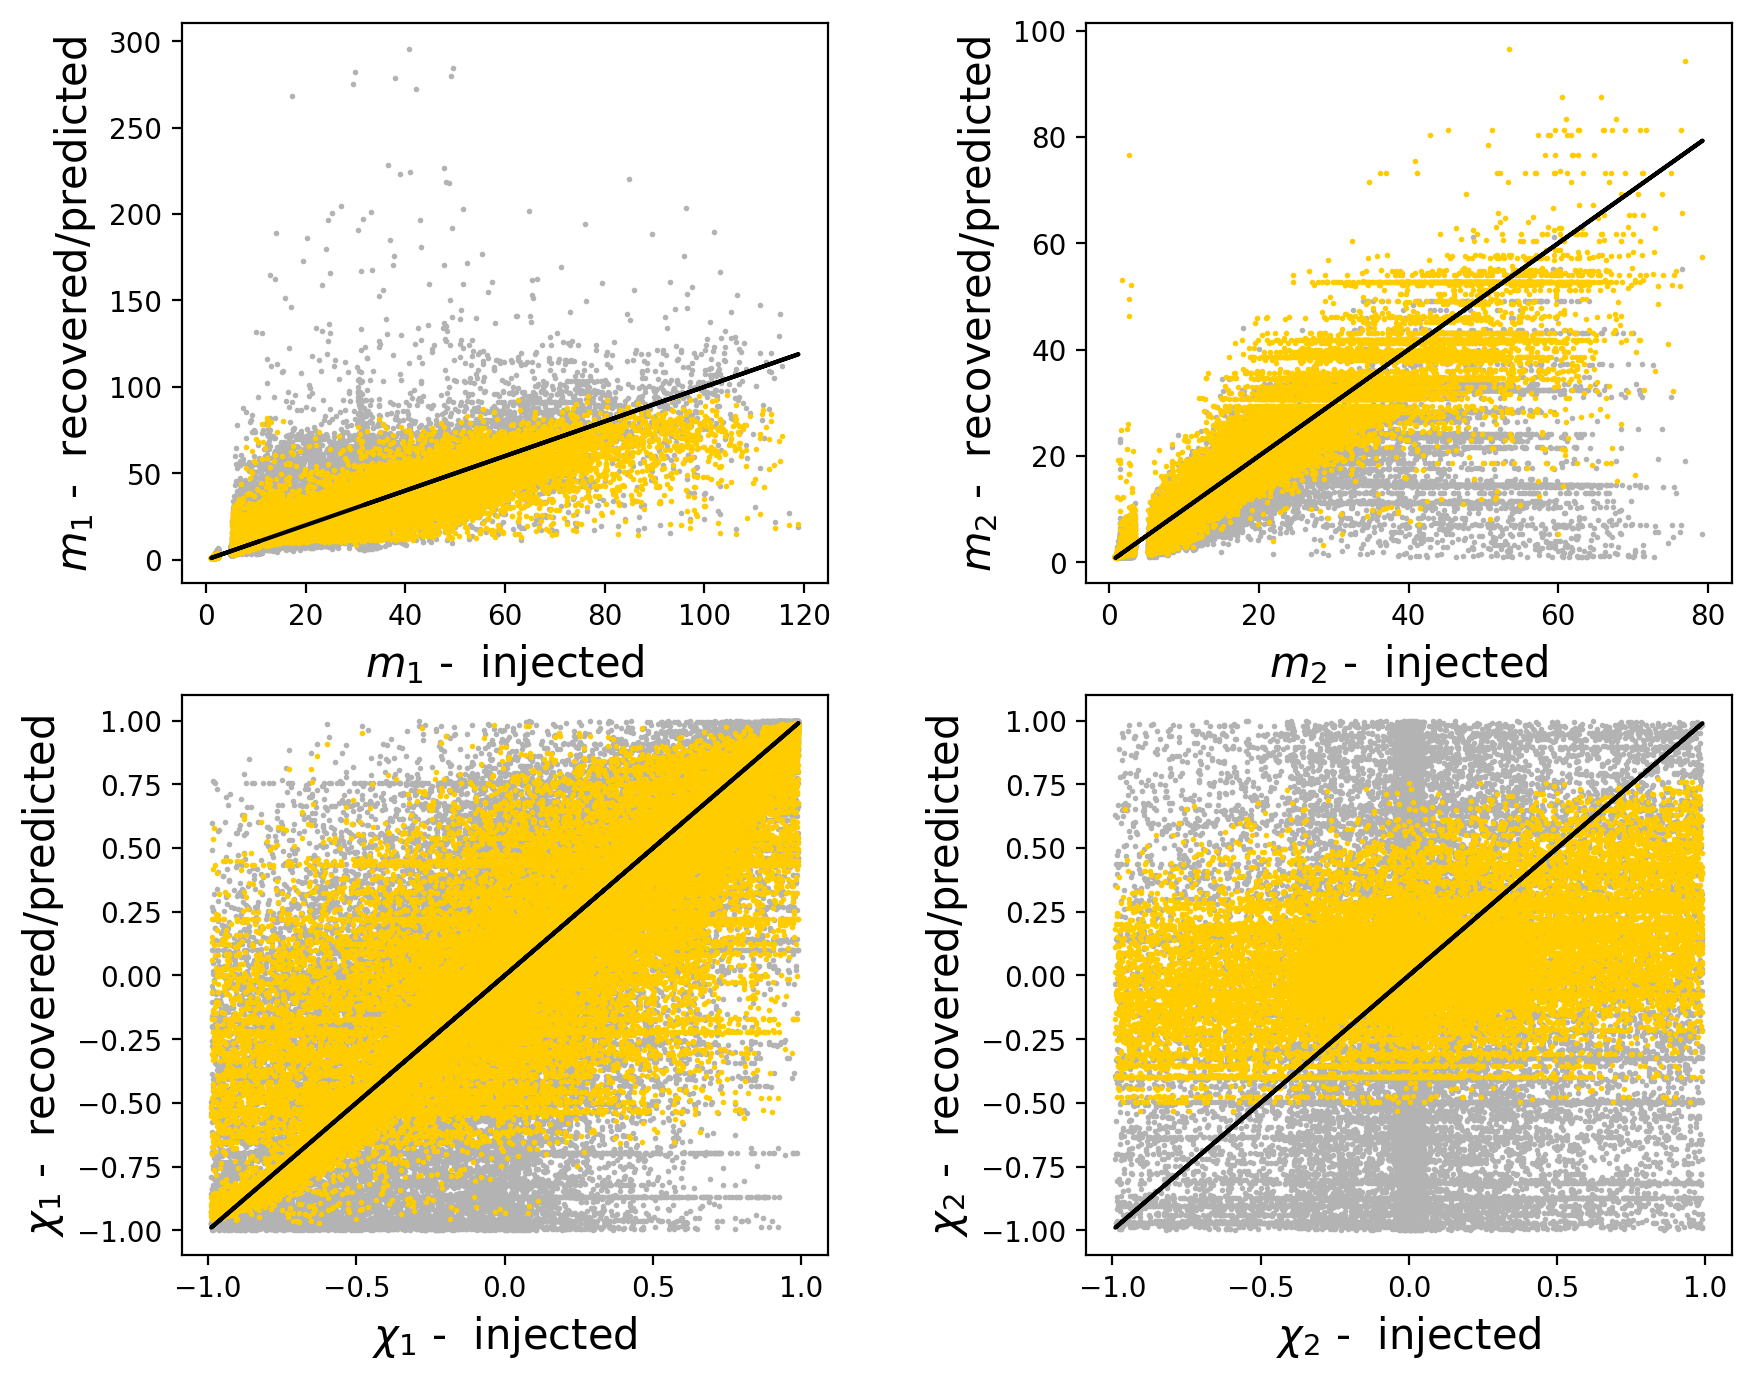
\includegraphics[width=0.45\textwidth]{m1m2chi1chi2_NN_recvspred.png}
%    \caption{NN version of Fig.~\ref{m_chi_comparisons}}
%        \label{m1m2chi1chi2_NN_recvspred}
%\end{figure}

%\begin{figure}
%% >> python3 paper_plots.py --NN -v --plots histo --histo_logs 1 1 0 0 --histo_fmin -10 -10 -2 -2
%    \centering
%    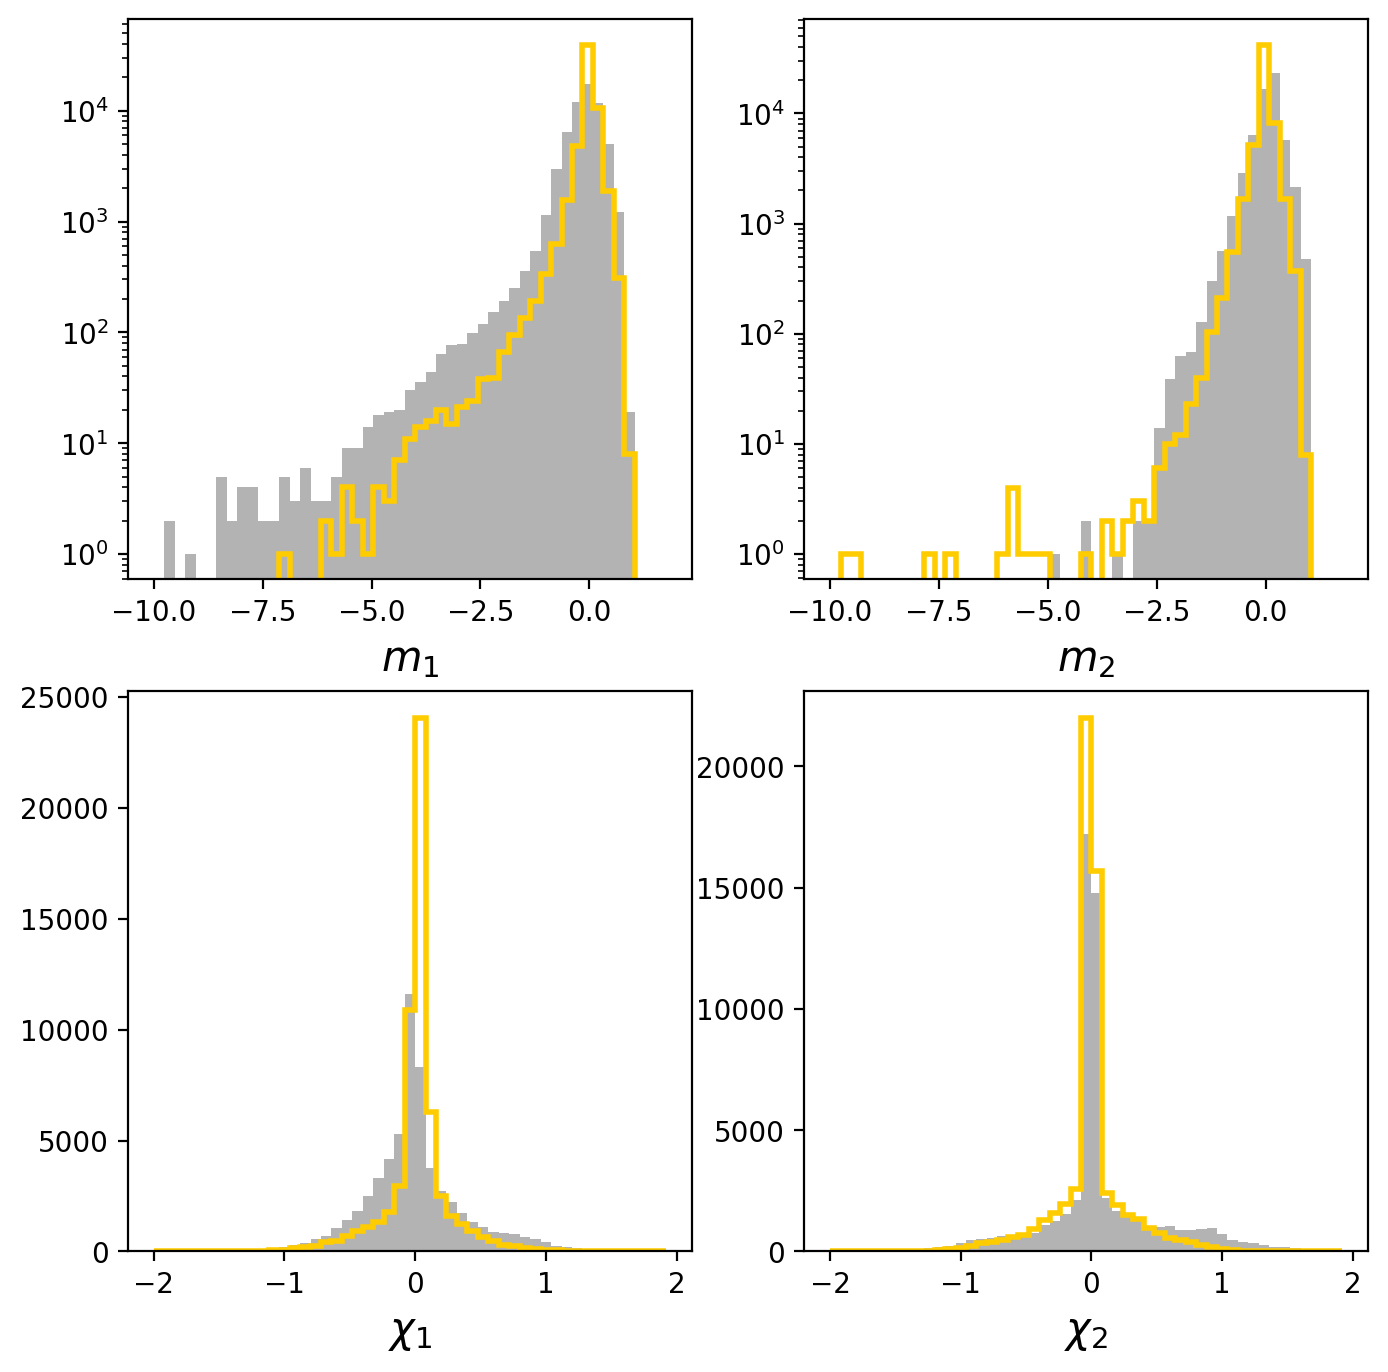
\includegraphics[width=0.45\textwidth]{m1m2chi1chi2_NN_histo.png}
%    \caption{Histograms}
%        \label{m1m2chi1chi2_NN_histo}
%\end{figure}

\begin{table*}
% >> python3 paper_plots.py --NN -v --errortab --tab_format tex --vars m1m2chi1chi2
  \caption{\label{tab:errors}  Mean differences in absolute value $|\Delta \bar{y}|=  \frac{1}{N} \Sigma |y^i_{\rm inj} - y^i_{\rm rec/pred}|$
  and averages of the relative
  differences in absolute value $|\delta \bar{y}| = \frac{1}{N} \Sigma \left( |y^i_{\rm inj} - y^i_{\rm rec/pred}|/y^i_{\rm inj} \right) $ for recovered and predicted data.
 The standard deviation  $\sigma^{\Delta y}$ and $\sigma^{\delta y}$ are computed, respectively, from the difference and relative difference distributions 
 without absolute value. Note that ${\cal{M}}_c$ is not directly predicted but it is computed from the predicted  masses $m_i$.}
  \begin{center}
  \begin{tabular}{c|cccc|cccc|cccc}
  \hline\hline
  & $|\Delta \bar{y}_{\rm rec}|$   & $\sigma_{\rm rec}^{\Delta y}$  & $|\delta \bar{y}_{\rm rec}|$  & $\sigma_{\rm rec}^{\delta y}$   &
      $|\Delta \bar{y}_{\rm nn}|$   & $\sigma_{\rm nn}^{\Delta y}$   & $|\delta \bar{y}_{\rm nn}|$   & $\sigma_{\rm nn}^{\delta y}$  &
      $|\Delta \bar{y}_{\rm gpr}|$  & $\sigma_{\rm gpr}^{\Delta y}$  & $|\delta \bar{y}_{\rm gpr}|$  & $\sigma_{\rm gpr}^{\delta y}$  \\
  \hline\hline
$m_1$          & $6.625$ & $12.052$ & $0.352$ & $0.596$ & $3.456$ & $6.976$ & $0.134$ & $0.292$ & 3.241 & ... & 0.127 & 0.279\\
$m_2$          & $2.761$ & $7.178$ & $0.256$ & $0.351$ & $1.457$ & $3.583$ & $0.123$ & $0.331$   &1.414  & ... & 0.111 & 0.319 \\
$\chi_1$       & $0.266$ & $0.388$ &  /  &  /  & $0.138$ & $0.236$ &  /  &  /  & 0.134 & 0.194 & / &  / \\
$\chi_2$       & $0.277$ & $0.460$ &  /  &  /  & $0.153$ & $0.268$ &  /  &  /  & 0.151 & 0.225 & / & / \\
\hline
${\cal{M}}_c$  & $1.323$ & $4.687$ & $0.039$ & $0.104$ & $0.769$ & $2.285$ & $0.036$ & $0.087$  & 0.712 & ... & 0.027 & 0.079\\
  \hline\hline
\end{tabular}
\end{center}
\end{table*}

